\thispagestyle{toancuabinone}
\pagestyle{toancuabi}
\everymath{\color{toancuabi}}
%\blfootnote{$^1$\color{toancuabi}Đại học Thăng Long.}
\graphicspath{{../toancuabi/pic/}}
\begingroup
\AddToShipoutPicture*{\put(0,616){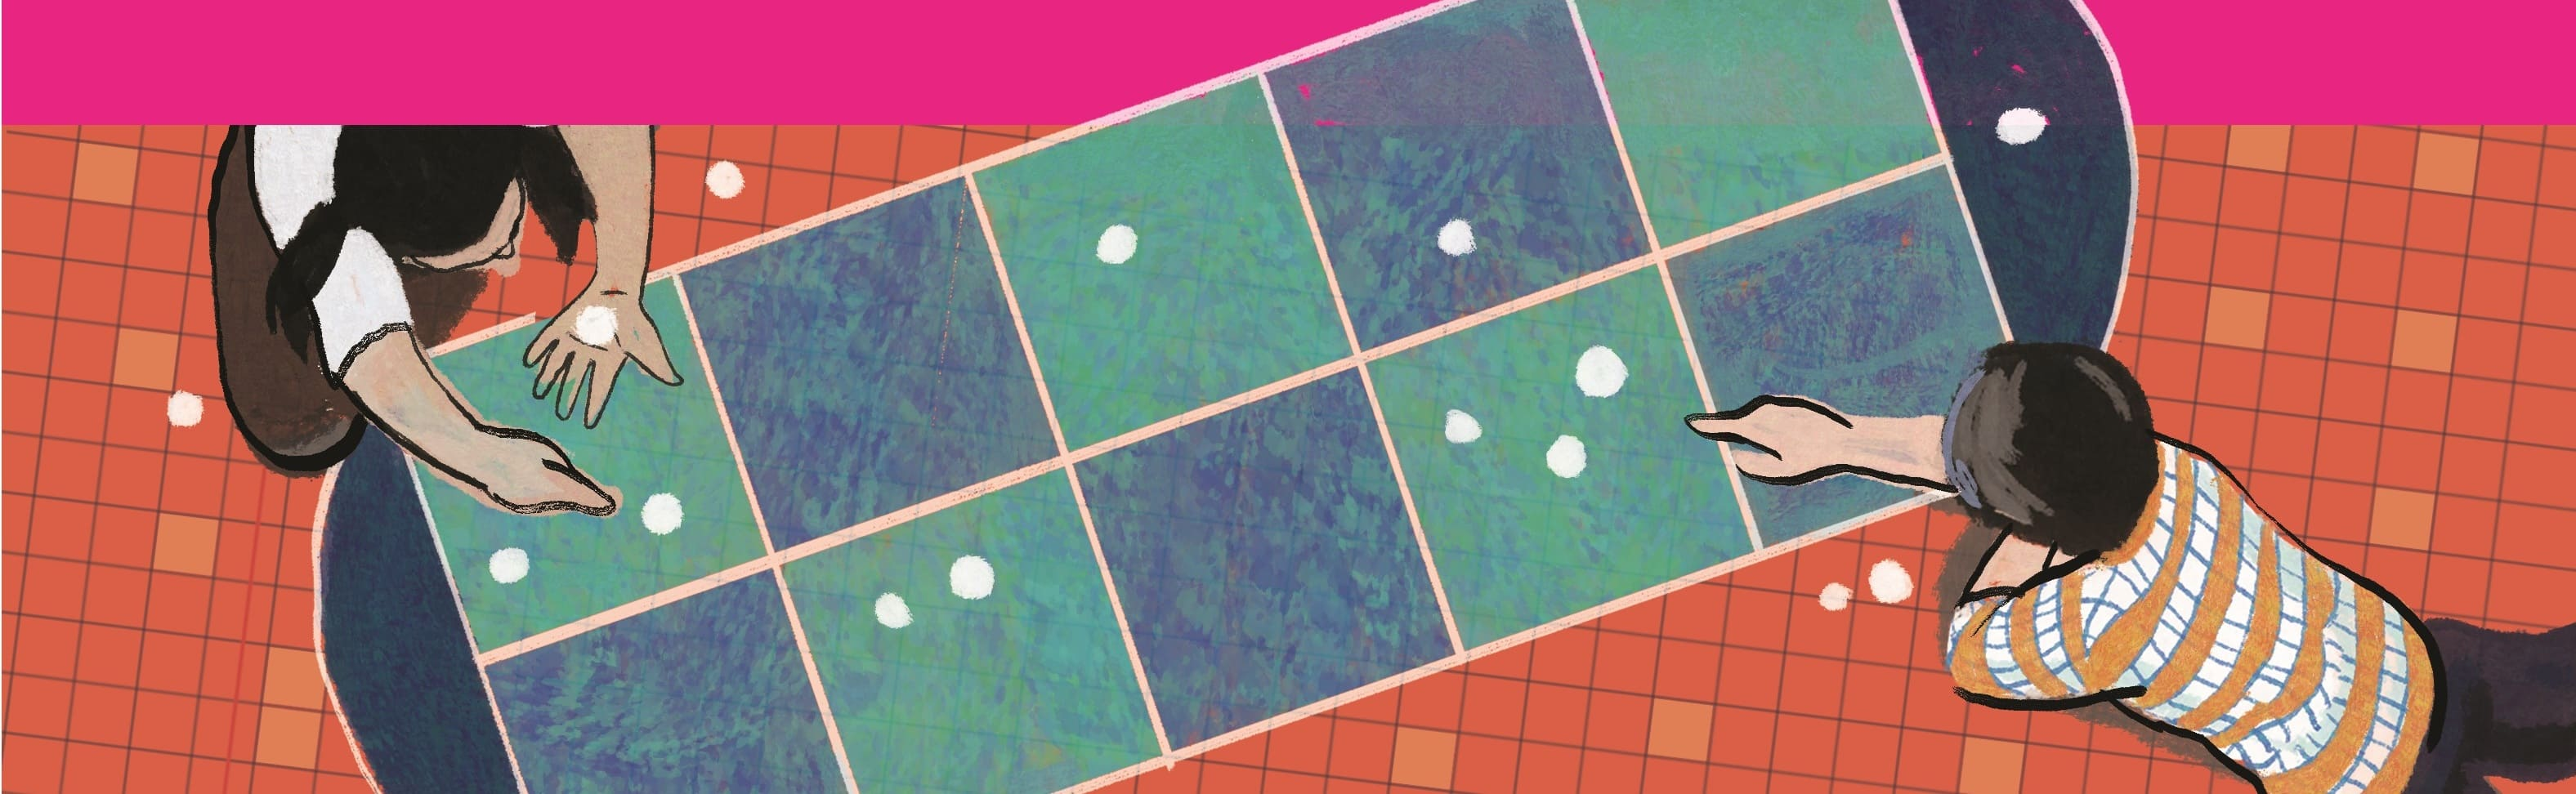
\includegraphics[width=19.3cm]{../bannertoancuabi}}}  
\AddToShipoutPicture*{\put(85,525){
\includegraphics[scale=1]{../tieude1.pdf}}} 
\centering
\endgroup

\vspace*{182pt}

\begin{multicols}{2}
	Mục Toán của Bi trong Số $11$, Tập $6$ đã giới thiệu đến các em cách tính diện tích của những hình tạo trên lưới ô vuông. Rất nhiều hình khác nhau có các đỉnh tại các điểm nguyên đều tính được mà chỉ cần dựa trên những ô vuông đơn vị có diện tích $1$. Không biết diện tích của những hình trên lưới có liên hệ gì với những điểm trên lưới không nhỉ? Định lý Pick được giới thiệu trong phần này sẽ trả lời cho ta câu hỏi rất thú vị này đấy.
	\vskip 0.1cm
	$\pmb{1.}$ \textbf{\color{toancuabi}Định lý Pick}
	\vskip 0.1cm
	Để xem diện tích của một hình trên lưới tính thế nào qua các điểm trên lưới (còn gọi là điểm nguyên), chúng ta thử tính diện tích của một hình cơ bản trong Phần $1$ -- hình chữ nhật kích thước $3\times4$ có các cạnh nằm trên các đường thẳng của lưới bằng một cách khác nhé. Bây giờ, ta chia hình chữ nhật đã cho bởi những đường thẳng song song, cách đều, đi qua giữa hai điểm nguyên trên các cạnh của hình chữ nhật như trong Hình $1$ dưới đây. 
	\begin{figure}[H]
		\vspace*{-5pt}
		\centering
		\captionsetup{labelformat= empty, justification=centering}
		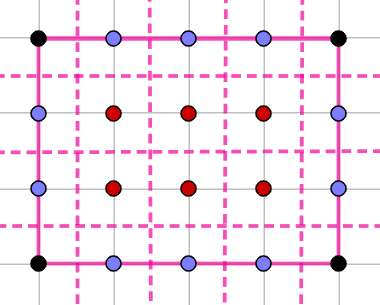
\includegraphics[width= 0.65\linewidth]{1}
		\caption{\small\textit{\color{toancuabi}Hình $1$.}}
		\vspace*{-5pt}
	\end{figure}
	Khi đó ta thấy
	\vskip 0.1cm
	-- Mỗi điểm nguyên ({\color{red}màu đỏ}) nằm trong hình chữ nhật ứng với một hình vuông đơn vị;
	\vskip 0.1cm
	-- Mỗi điểm nguyên ({\color{blue}màu xanh dương}) nằm trên các cạnh của hình chữ nhật mà không phải đỉnh ứng với một nửa hình vuông đơn vị;
	\vskip 0.1cm
	Mỗi điểm nguyên là đỉnh ({\color{black}màu đen}) của hình chữ nhật ứng với một phần tư hình vuông đơn vị.
	\vskip 0.1cm
	Như vậy
	\vskip 0.1cm
	Diện tích của hình chữ nhật $=$ số điểm trong hình chữ nhật
	$+ \dfrac{1}{2}\times$ số điểm trên cạnh mà không phải đỉnh $+ \dfrac{1}{4}\times$ số đỉnh
	\vskip 0.1cm
	Do hình chữ nhật có $4$ đỉnh nên ta thấy ngay
	\vskip 0.1cm
	Diện tích của hình chữ nhật $=$ số điểm trong hình chữ nhật 
	$+ \dfrac{1}{2} \times$ số điểm nằm trên cạnh
	$- 1$.
	\vskip 0.1cm
	Từ đó ta có diện tích của hình chữ nhật trên là:
	\begin{align*}
		6 + \frac{1}{2}\times14 - 1 = 12 \text{ (đơn vị diện tích).}
	\end{align*}
	Ví dụ trên được tính trong một trường hợp cụ thể, tuy nhiên những lập luận này hoàn toàn có thể áp dụng cho tất cả những hình chữ nhật khác cùng đặc điểm. Như vậy diện tích của hình chữ nhật có các cạnh trùng với những đường thẳng của lưới có thể được tính thông qua số điểm nguyên nằm trong và nằm trên cạnh của hình chữ nhật. Nếu ta gọi $T$ là số điểm nằm trong và $B$ là số điểm nằm trên các cạnh của hình chữ nhật, thì diện tích của hình chữ nhật là:
	\begin{align*}
		T+  \frac{B}{2} - 1.
	\end{align*}
	Một công thức thật đơn giản, thật hay đúng không các em. Không biết ngoài hình chữ nhật, công thức tính diện tích này còn đúng với những hình nào nữa nhỉ?
	\vskip 0.1cm
	Chúng ta cùng xem xét diện tích hình cơ bản thứ hai được đề cập trong Phần $1$ -- tam giác vuông có hai cạnh góc vuông trùng với những đường thẳng của lưới.
	\begin{figure}[H]
		\vspace*{-5pt}
		\centering
		\captionsetup{labelformat= empty, justification=centering}
		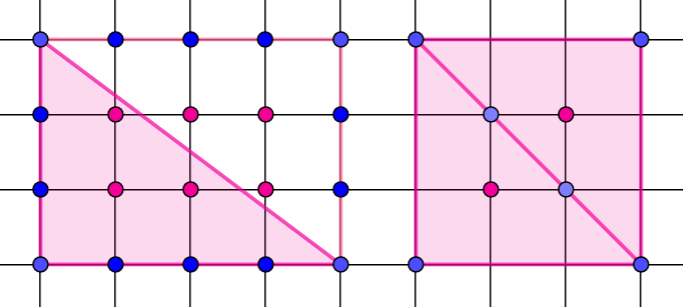
\includegraphics[width= 0.7\linewidth]{2}
		\caption{\small\textit{\color{toancuabi}Hình $2$.}}
		\vspace*{-10pt}
	\end{figure}
	Bây giờ ta kẻ hình chữ nhật bao quanh tam giác vuông và dùng công thức tính diện tích qua các điểm của hình chữ nhật được chỉ ra ở trên để xem về công thức tính diện tích của tam giác.
	\vskip 0.1cm
	Giả sử trên cạnh huyền của tam giác vuông có $d$ điểm nguyên. Nhận thấy $d$ điểm này vẫn là điểm trong của hình chữ nhật bao quanh. Do đó
	\vskip 0.1cm
	Số điểm trong $t$ của hình tam giác $= \dfrac{1}{2} \times $ (số điểm trong $T$ của hình chữ nhật $-$ số điểm trên cạnh huyền $d$)
	\vskip 0.1cm
	Hay $T = 2\times t + d$.
	\vskip 0.1cm
	Mặt khác, do tính đối xứng nên số điểm nguyên nằm trên hai cạnh góc vuông của tam giác vuông đã cho và tam giác vuông bù với nó, nên ta lại có
	\vskip 0.1cm
	Số điểm biên $b$ của hình tam giác $= \dfrac{1}{2} \times$ số điểm biên $B$ của hình chữ nhật 
	$+ 1$ điểm đỉnh $+$ số điểm trên cạnh huyền $d$.
	\vskip 0.1cm
	Hay $B = 2i - 2d - 2$.
	\vskip 0.1cm
	Vậy từ công thức tính diện tích của hình chữ nhật, ta có
	\vskip 0.1cm
	Diện tích tam giác vuông $= \dfrac{1}{2}$ diện tích hình chữ nhật
	$= \dfrac{T}{2} + \dfrac{B}{4} - \dfrac{1}{2}$
	$= t + \dfrac{b}{2} - 1$.
	\vskip 0.1cm
	Như vậy là công thức tính diện tích qua các điểm cũng đúng tiếp tam giác vuông! Đến đây, hẳn nhiều bạn nhỏ tiếp tục đặt câu hỏi: Công thức tính diện tích qua các điểm còn đúng cho dạng hình nào trên lưới nữa nhỉ? Câu hỏi này của chúng ta đã được một nhà toán học người Áo là Georg Alexander Pick ($1859 - 1942$) đưa ra câu trả lời. Ông đã chứng minh được Công thức tính diện tích qua những điểm nguyên đúng cho các đa giác đơn có các đỉnh là các điểm trên lưới. Kết quả này được phát biểu qua định lý mang tên ông -- Định lý Pick.
	\vskip 0.1cm
	\textbf{\color{toancuabi}Định lý Pick:} Cho một đa giác đơn có các đỉnh là các điểm nguyên của một lưới ô vuông. Giả sử có $T$ điểm nằm trong đa giác và $B$ điểm nằm trên các cạnh của đa giác (bao gồm cả các đỉnh). Khi đó diện tích của đa giác là:
	\begin{align*}
		T+  \dfrac{B}{2}-1.
	\end{align*}
	Một lưu ý là Định lý Pick tính diện tích cho những hình là đa giác đơn, là những đa giác không có cạnh tự cắt các em nhé. Dưới đây là một vài minh họa cho những đa giác loại này.
	\begin{figure}[H]
		\vspace*{-5pt}
		\centering
		\captionsetup{labelformat= empty, justification=centering}
		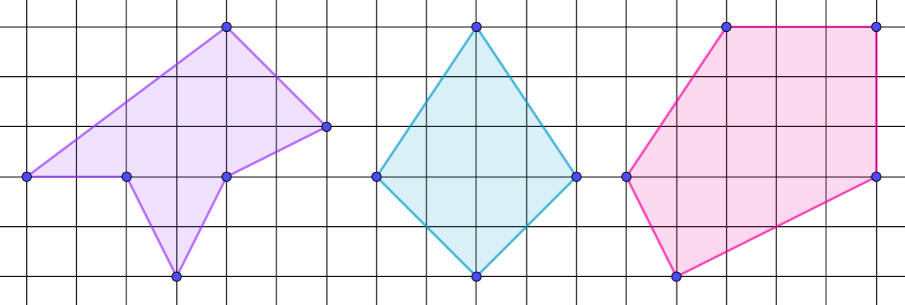
\includegraphics[width= 1\linewidth]{3}
		\caption{\small\textit{\color{toancuabi}Hình $3$. Đa giác đơn.}}
		\vspace*{-5pt}
	\end{figure}
	\begin{figure}[H]
		\vspace*{5pt}
		\centering
		\captionsetup{labelformat= empty, justification=centering}
		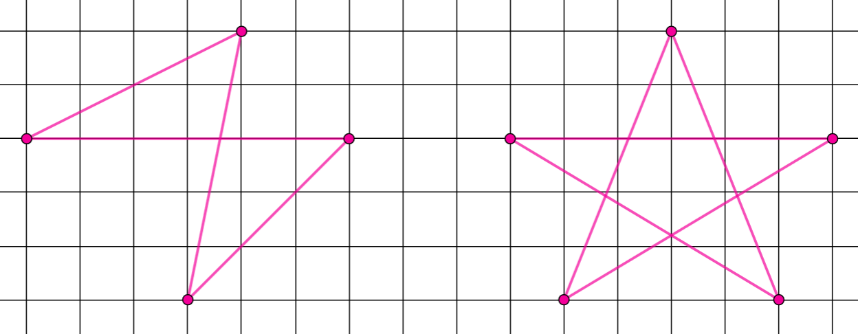
\includegraphics[width= 1\linewidth]{4}
		\caption{\small\textit{\color{toancuabi}Hình $4$. Đa giác không đơn.}}
		\vspace*{-10pt}
	\end{figure}
	Việc áp dụng định lý cho các đa giác không đơn có thể dẫn đến kết quả không chính xác. Các em ghi nhớ điều này khi dùng định lý Pick để tính diện tích nhé.
	\begin{figure}[H]
		\vspace*{-5pt}
		\centering
		\captionsetup{labelformat= empty, justification=centering}
		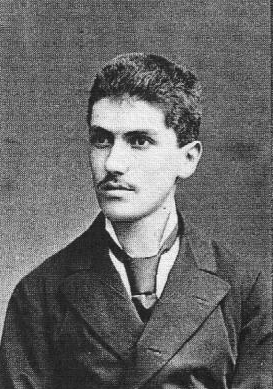
\includegraphics[width= 0.55\linewidth]{5}
		\caption{\small\textit{\color{toancuabi}Hình $5$. Georg Alexander Pick.}}
		\vspace*{-10pt}
	\end{figure}
	Định lý Pick được phát biểu đầy đủ như sau.
	\vskip 0.1cm
	$\pmb{2.}$ \textbf{\color{toancuabi}Tính diện tích theo định lý Pick}
	\vskip 0.1cm
	Trong mục này, chúng ta tính lại diện tích của một số hình trong Phần $1$ theo công thức có được từ định lý Pick và so sánh với nhau nhé.
	Đầu tiên là ``chú mèo" đáng yêu trong Ví dụ $4$ của Phần $1$.
	\vskip 0.1cm
	\textbf{\color{toancuabi}Ví dụ} $1$. Tính diện tích của hình được tô đậm dưới đây.
	\begin{figure}[H]
		\vspace*{-5pt}
		\centering
		\captionsetup{labelformat= empty, justification=centering}
		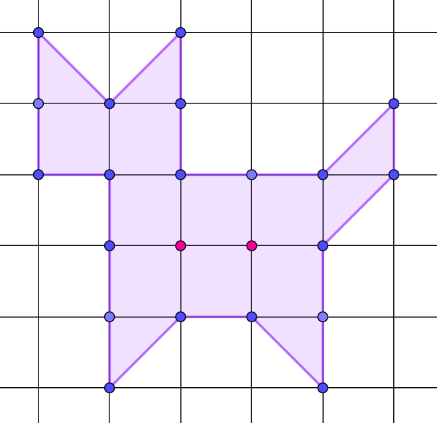
\includegraphics[width= 0.45\linewidth]{6}
		\caption{\small\textit{\color{toancuabi}Hình $6$.}}
		\vspace*{-10pt}
	\end{figure}
	\textit{Lời giải.} Ta dễ dàng thấy ngay $T = 2$ điểm trong ``chú mèo" và $B = 20$ điểm nằm trên các cạnh biên. Từ đó, diện tích của ``chú mèo" là:
	\begin{align*}
		T + \frac{B}{2} - 1 = 2 + \frac{20}{2} - 1 = 11 \text{ (đơn vị diện tích)}.
	\end{align*}
	Kết quả này cũng giống với con số mà ta đã tính được trong Phần $1$, nhưng có phần nhanh chóng hơn các em nhỉ.
	\vskip 0.1cm
	Chúng ta thử tiếp với hình trong Ví dụ $6$ trong Phần $1$.
	\vskip 0.1cm
	\textbf{\color{toancuabi}Ví dụ} $\pmb{2.}$ Tính diện tích của đa giác được tô đậm trong hình sau.
	\begin{figure}[H]
		\vspace*{-5pt}
		\centering
		\captionsetup{labelformat= empty, justification=centering}
		
\includegraphics[width= 0.55\linewidth]{7}
		\caption{\small\textit{\color{toancuabi}Hình $7$.}}
		\vspace*{-10pt}
	\end{figure}
	\textit{Lời giải.}	Đa giác trong Hình $7$ có $T = 8$ điểm trong và $B = 6$ điểm nằm trên các canh. Do đó, Định lý Pick cho ta diện tích của đa giác này là:
	\begin{align*}
		T + \frac{B}{2} - 1 = 10 \text{ (đơn vị diện tích).}
	\end{align*}
	Kết quả này tất nhiên là trùng với con số tính ra theo cách giới thiệu ở Phần $1$ rồi, nhưng thay vì phải tính khá nhiều diện tích tam giác thông qua phương pháp lấy phần bù, chúng ta chỉ cần đếm số điểm nằm trên lưới. Định lý Pick thật là lợi hại phải không!
	\vskip 0.1cm
	Bài tập dưới đây để các em luyện tập thêm công thức Pick. Các em có thể tính diện tích theo cách trong Phần $1$ để kiểm tra lại nhé.
	\vskip 0.1cm
	\textbf{\color{toancuabi}Bài tập} $\pmb{1.}$ Tính diện tích của hình tô đậm sau đây.
	\begin{figure}[H]
		\vspace*{-5pt}
		\centering
		\captionsetup{labelformat= empty, justification=centering}
		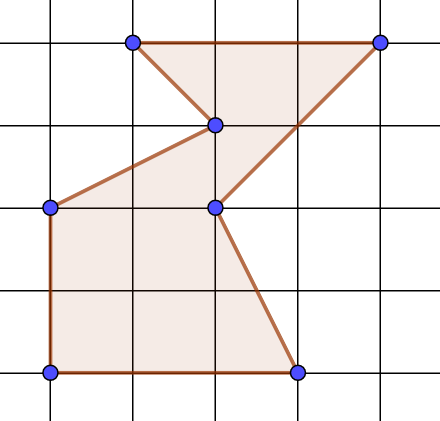
\includegraphics[width= 0.35\linewidth]{8}
		\caption{\small\textit{\color{toancuabi}Hình $8$.}}
		\vspace*{-5pt}
	\end{figure}
	$\pmb{3.}$ \textbf{\color{toancuabi}Làm thế nào để chứng minh định lý Pick?}
	\vskip 0.1cm
	Định lý Pick có thể chứng minh bằng nhiều cách khác nhau, trong khuôn khổ bài viết này, chúng ta chỉ mô tả cách tìm ra công thức của Pick cho hai hình cơ bản, đơn giản nhất -- hình chữ nhật và tam giác vuông có cạnh nằm trên lưới.
	\vskip 0.1cm 
	Nếu bạn nào quan tâm đến việc chứng minh đầy đủ định lý này thì có thể tham khảo các bước làm sau.
	\vskip 0.1cm
	-- Để chứng minh công thức Pick cho một đa giác nào đó ta chia đa giác thành hai phần bằng một đường chéo và quy về việc chứng công thức Pick cho mỗi đa giác thành phần. Ta thấy, đường chéo này trở thành cạnh của hai đa giác thành phần do đó các điểm nguyên trên đường chéo lúc trước được tính $1$ đơn vị, khi trở thành điểm biên thì tính $\dfrac{1}{2}$ đơn vị nhưng tính hai lần, vậy là hòa! Còn lại là hai điểm mút của đường chéo, chúng được tính hai lần do là đỉnh của hai đa giác con, vậy là dôi ra $1$ đơn vị. Nhưng trong công thức Pick sau khi tính các điểm biên và điểm trong ta bớt đi $1$ đơn vị. Đối với hai đa giác thành phần, ta bớt đi cả thảy $2$ đơn vị, vậy cũng hòa! 
	\begin{figure}[H]
		\vspace*{-5pt}
		\centering
		\captionsetup{labelformat= empty, justification=centering}
		
\includegraphics[width= 0.45\linewidth]{9}
		\caption{\small\textit{\color{toancuabi}Hình $9$.}}
		\vspace*{-10pt}
	\end{figure}
	-- Sau khi thực hiện nhiều lần chia đa giác thành các đa giác con, cuối cùng ta quy việc chứng minh định lý Pick cho tam giác. Ta lại tiếp tục chia tam giác đó thành các tam giác con nếu có một điểm nguyên ở trong hoặc trên biên tam giác. 
	\begin{figure}[H]
		\vspace*{5pt}
		\centering
		\captionsetup{labelformat= empty, justification=centering}
		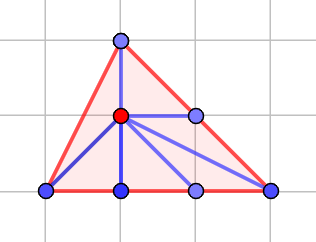
\includegraphics[width= 0.4\linewidth]{10}
		\caption{\small\textit{\color{toancuabi}Hình $10$.}}
		\vspace*{-10pt}
	\end{figure}
	-- Đối với tam giác không chứa điểm nguyên ở trong hoặc trên biên, định lý Pick khẳng định nó có diện tích bằng
	\begin{align*}
		\dfrac{3}{2}-1=\dfrac{1}{2} \text{ (đơn vị diện tích).}
	\end{align*}
	Dưới đây chúng ta sẽ xem một vài ví dụ kiểm chứng điều này. Hy vọng sau đó các bạn có thể tự đưa ra một chứng minh chặt chẽ của định lý Pick cho các tam giác đơn (nghĩa là tam giác không chứa điểm nguyên ở trong và trên biên, ngoại từ ba đỉnh).
	\begin{figure}[H]
		\vspace*{-5pt}
		\centering
		\captionsetup{labelformat= empty, justification=centering}
		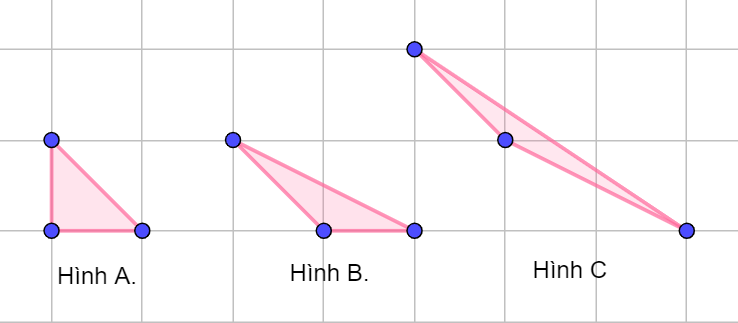
\includegraphics[width= 1\linewidth]{11}
		\caption{\small\textit{\color{toancuabi}Hình $11$.}}
		\vspace*{-10pt}
	\end{figure}
	Ba tam giác trong Hình $11$ đều là các tam giác đơn. Ba tam giác này có nhiều hình dáng khác nhau, nhưng ta đều thấy chúng có diện tích bằng $\dfrac{1}{2}$.
	Thật vậy, vận dụng những cách tính diện tích trong Phần $1$, ta có thể thấy ngay
	\begin{figure}[H]
		\vspace*{-5pt}
		\centering
		\captionsetup{labelformat= empty, justification=centering}
		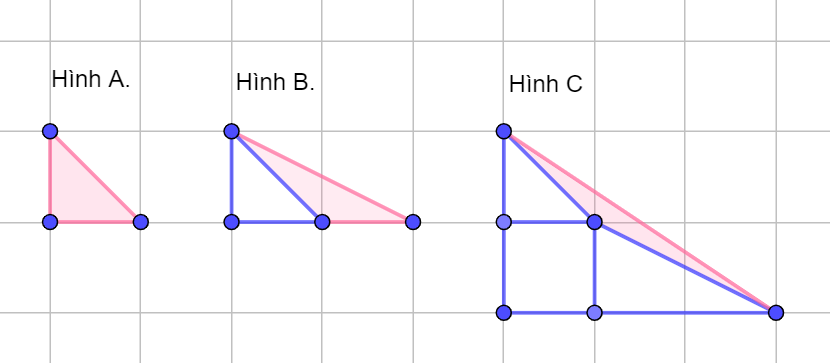
\includegraphics[width= 1\linewidth]{12}
		\caption{\small\textit{\color{toancuabi}Hình $12$.}}
		\vspace*{-10pt}
	\end{figure}
	-- Diện tích tam giác trong Hình $A$ là $\dfrac{1}{2}$;
	\vskip 0.1cm
	Diện tích của tam giác trong Hình $B$ là: 
	\begin{align*}
		\dfrac{1}{2}\times 1\times 2 - \dfrac{1}{2} = \dfrac{1}{2};
	\end{align*}
	Diện tích của tam giác trong Hình $C$ là: 
	\begin{align*}
		\dfrac{1}{2}\times2\times3 - \dfrac{1}{2} - 1 - \dfrac{1}{2}\times1\times2 = \dfrac{1}{2}.
	\end{align*}
	Bài viết về Tính diện tích trên lưới ô vuông đã giới thiệu đến các em cách tính diện tích của những hình trên lưới. Đầu tiên là hai phương pháp rất phổ biến: phương pháp chia hình cần tính thành những hình cơ bản đã biết diện tích và phương pháp tính theo phần bù. Tiếp theo đó bài viết giới thiệu với các em một công thức tính diện tích vô cùng đẹp đẽ qua Định lý Pick. Việc áp dụng định lý Pick giúp tính diện tích trở nên đơn giản hơn nhiều vì ta chỉ cần đếm số điểm nguyên ở trong và trên cạnh của hình cần tính. Chủ đề tính diện tích trên lưới ô vuông vẫn còn nhiều điều hấp dẫn, các bạn nhỏ nếu tìm được những bài toán hay thì hãy chia sẻ cùng Pi và các thầy cô trong câu lạc bộ UMC nhé.
\end{multicols}

%\begin{multicols}{2}
%	Thám tử Xuân Phong trong một lần đi du lịch cùng thanh tra Lê Kính tới một hòn đảo xa xôi tận bên Phi Châu được đặt chân tới một ngôi làng đẹp tuyệt diệu ẩn sau những cành cọ, rặng dừa xum xuê chạy dài bờ biển xanh ngắt trong veo. Trưởng làng đon đả mời hai người tới ngôi nhà lớn của cả làng để dự một lễ hội đặc biệt của người dân. Theo như chỉ dẫn từ công ty lữ hành, những người thổ dân ở làng đó chia thành hai họ tộc, họ Tutu chuyên nói thật và họ Titi lại chuyên nói dối. Khi bước vào căn nhà lớn, Xuân Phong đã thấy có $50$ người dân đảo ăn mặc\hspace*{123pt}\linebreak[6]những bộ quần\hspace*{123pt}\linebreak[6]áo màu sắc lộng\hspace*{123pt}\linebreak[6]lẫy dành riêng\hspace*{123pt}\linebreak[6]cho lễ hội và\hspace*{123pt}\linebreak[6]ngồi xung quanh\hspace*{123pt}\linebreak[6]một chiếc bàn\hspace*{123pt}\linebreak[6]tròn thật to đặt\hspace*{123pt}\linebreak[6]giữa phòng. Theo\hspace*{123pt}\linebreak[6]như tục lệ, $50$\hspace*{123pt}\linebreak[6]người sẽ lần lượt\hspace*{123pt}\linebreak[6]đứng lên và nếu\hspace*{123pt}\linebreak[6]số tuổi của hai\hspace*{123pt}\linebreak[6]người ngồi cạnh\hspace*{123pt}\linebreak[6]anh ta, tuổi\hspace*{123pt}\linebreak[6]người ngồi bên\hspace*{123pt}\linebreak[6]trái trước -- sau\hspace*{123pt}\linebreak[6]đó là người ngồi\hspace*{123pt}\linebreak[6]bên phải. Xuân\hspace*{123pt}\linebreak[6]Phong được biết trước trong sách hướng dẫn du lịch là: người tộc Tutu sẽ nói đúng cả hai con số này, còn người tộc Titi sẽ tăng một trong hai số tuổi của hai người ngồi cạnh (người nào theo cách anh ta tùy thích chọn) thêm $1$ tuổi còn giảm tuổi kia đi $1$ tuổi. Xuân Phong chỉ cần nghe xong và ghi chép lại $50$ câu nói  của $50$ người dân làng ngồi quanh bàn, sau một chút suy nghĩ, đã biết được ngay ai là người đến từ tộc nào, Tutu hay Titi. Làm sao mà thám tử lại tài thế nhỉ, các em có biết cách lập luận của Xuân Phong được hay không?
%	
%	\vspace*{280pt}
%	\insertpic{159}{85}{0.54}{xp}
%\end{multicols}
%\newpage
%\begingroup
%\AddToShipoutPicture*{\put(112,672){
\includegraphics[scale=1]{../tieude11.pdf}}} 
%\centering
%\endgroup
%\vspace*{35pt}
%
%\begin{multicols}{2}
%	$\pmb{1.}$ Bạn Tùng làm một số bài trắc nghiệm và sau đó sẽ lấy điểm trung bình của các bài đó để tự đánh giá học lực của mình. Trả lời xong bài trắc nghiệm cuối cùng, Tùng thấy rằng nếu bài này mình được $97$ điểm bài này thì điểm trung bình của tất cả các bài trắc nghiệm sẽ là $90$ điểm, còn nếu như ở bài cuối Tùng chỉ nhận được $73$ điểm thì điểm trung bình của bạn ấy sẽ chỉ còn $87$ điểm. Vậy số bài trắc nghiệm trong loạt bài mà Tùng đã làm là bao nhiêu?
%	\begin{figure}[H]
%		\centering
%		\vspace*{-10pt}
%		\captionsetup{labelformat= empty, justification=centering}
%		\includegraphics[width=0.95\linewidth]{Pi12_Bai1}
%		\vspace*{-10pt}
%	\end{figure}
%	\vskip 0.1cm
%	$\pmb{2.}$ Có $3$ loại kẹo để trong lọ thủy tinh với ba màu khác nhau: kẹo màu đỏ, kẹo màu vàng và kẹo màu trắng. Nếu Bình nhặt hết số kẹo màu vàng thì tổng số kẹo trong lọ ít hơn một chiếc so với $2/3$ tổng số kẹo ban đầu. Còn nếu Bình nhặt hết số kẹo đỏ, thì số kẹo còn lại trong lọ nhiều hơn $4$ chiếc so với $2/3$ tổng số kẹo ban đầu.
%	\vskip 0.1cm
%	Vậy ban đầu trong hai loại kẹo màu vàng và kẹo màu trắng, loại nào có nhiều và nhiều hơn bao nhiêu?
%	\begin{figure}[H]
%		\centering
%		\vspace*{-10pt}
%		\captionsetup{labelformat= empty, justification=centering}
%		\includegraphics[width=0.45\linewidth]{Pi12_Bai2}
%		\vspace*{-15pt}
%	\end{figure}
%	$\pmb{3.}$ $40$ bạn nhỏ nắm tay nhau xếp thành vòng tròn quanh đống lửa trại. Có tất cả $22$ bạn có nắm tay một bạn nam, và $30$ bạn có nắm tay một bạn nữ. Hỏi có tất cả bao nhiêu bạn nữ xếp trong vòng tròn quanh lửa trại ngày hôm đó?
%	\begin{figure}[H]
%		\centering
%		\vspace*{-10pt}
%		\captionsetup{labelformat= empty, justification=centering}
%		\includegraphics[width=0.9\linewidth]{Pi12_Bai3}
%		\vspace*{-10pt}
%	\end{figure}
%	$\pmb{4.}$ Trên mặt bàn có $5$ đồng xu xếp thành hàng ngang. Đồng xu ở giữa đặt xấp còn $4$ đồng còn lại đều đặt ngửa. Mỗi một lần em được cho phép lật $3$ đồng xu đặt liền nhau tùy ý. Liệu em có thể có cách lật thế nào để cuối cùng $5$ đồng xu đều đặt xấp được không?
%	\vskip 0.1cm
%	Cũng câu hỏi như vậy, nếu lúc đầu đồng xu đặt xấp duy nhất là đồng xu xếp đầu hàng? Là đồng xu xếp thứ hai trong hàng?
%	\begin{figure}[H]
%		\centering
%		\vspace*{-5pt}
%		\captionsetup{labelformat= empty, justification=centering}
%		\includegraphics[width=1\linewidth]{Pi12_Bai4}
%		\vspace*{-20pt}
%	\end{figure}
%	$\pmb{5.}$ Một lần Lý Toét diện guốc mộc loẹt quẹt ra tận chợ phiên chơi ngày cuối tuần. Khi về nhà, Lý Toét ba hoa khoe khắp làng ``Tôi là tôi gặp $15$ ông bán cây cảnh ngoài chợ nhé. Mà tôi đi lòng vòng và nghiệm thấy cứ $3$ ông bất kỳ có tổng cộng đúng $10$ cây hoa hồng. Thế là tôi lẩm nhẩm đoán được ngay $15$ ông này có tất cả bao nhiêu cây hoa hồng."
%	\vskip 0.1cm
%	Em có thể đoán được như Lý Toét xem $15$ ông bán cây có tất cả bao nhiêu cây hoa hồng không? Hay Lý Toét có khoác lác hay nhầm lẫn gì không nhỉ?
%	\begin{figure}[H]
%		\centering
%%		\vspace*{1pt}
%		\captionsetup{labelformat= empty, justification=centering}
%		\includegraphics[width=0.58\linewidth]{Pi12_Bai5}
%		\vspace*{-15pt}
%	\end{figure}
%	$\pmb{6.}$ Có $20$ bạn tham gia nhóm Toán ngồi xung quanh một chiếc bàn tròn. Một lúc sau các bạn nhóm Văn cũng đến, cứ xen kẽ hai bạn nhóm Toán ngồi kề nhau giờ có thêm $20$ bạn mới từ nhóm Văn. Tổng cộng có tất cả $400$ bạn từ nhóm Văn ngồi thêm quanh chiếc bàn tròn rộng đó. Thỉnh thoảng một bạn nhóm Văn lại đứng dậy và rời khỏi bàn, dắt theo hai bạn ngồi cạnh mình đi luôn. Cứ như vậy, sau một lúc thì quanh bàn số bạn nhóm Toán còn lại chỉ là $3$ bạn. Hỏi số bạn nhóm Văn còn ở lại quanh bàn lúc đó ít nhất phải là bao nhiêu?
%\end{multicols}
%\vspace*{-12pt}
%\rule{1\linewidth}{0.1pt}
%\begingroup
%\AddToShipoutPicture*{\put(112,452){
\includegraphics[scale=1]{../tieude2.pdf}}} 
%\centering
%\endgroup
%\graphicspath{{../toancuabi/pic/}}
%\vspace*{80pt}
%
%\begin{multicols}{2}
%	$\pmb{1.}$ Có $30$ bạn học sinh tham gia một cuộc thi hùng biện bằng tiếng Anh. Các bạn lần lượt chọn các câu hỏi và trả lời theo thứ tự xếp hàng. Bạn thứ nhất được $80$ điểm, bạn thứ hai được $60$ điểm, bạn thứ ba có số điểm bằng trung bình cộng của bạn thứ nhất và bạn thứ hai, bạn thứ tư có số điểm bằng trung bình cộng của ba bạn đầu tiên. Nói chung, kể từ bạn thứ ba trở đi thì  mỗi một bạn học sinh tiếp theo luôn có số điểm bằng trung bình cộng số điểm của các bạn đã thi trước đó. 
%	\vskip 0.1cm
%	Hỏi bạn cuối cùng, tức bạn có số thứ tự $30$, đạt được bao nhiêu điểm trong cuộc thi? 
%	\begin{figure}[H]
%		\centering
%		\vspace*{-10pt}
%		\captionsetup{labelformat= empty, justification=centering}
%		\includegraphics[width=0.92\linewidth]{bai1}
%		\vspace*{-10pt}
%	\end{figure}
%	\textit{Lời giải.} 	Ta nhận thấy nếu mỗi bạn tiếp theo nhận được số điểm là trung bình cộng điểm số của các bạn đứng trước đó, thì trung bình cộng số điểm của các bạn luôn không thay đổi. Nếu hai bạn đầu tiên có trung bình cộng số điểm là $70$, thì kể từ bạn thứ ba, trung bình cộng số điểm của $n$ bạn đầu tiên, ($2\!<\!n\!<\!30$), luôn bằng $70$. Vì thế bạn cuối cùng cũng nhận được $70$ điểm.
%	\vskip 0.1cm
%	$\pmb{2.}$ Vào một ngày hè, ba bạn Yến, Vinh và Công đến hiệu kem và mỗi bạn đều lấy đủ $3$ vị: trái cây, vani và sô--cô--la (mỗi vị một cốc). Sau khi ăn xong, vì $3$ cốc cho một người là chưa đủ, nên Yến lấy thêm một cốc kem trái cây, Vinh lấy thêm một cốc kem vani và Công lấy thêm một cốc kem sô--cô--la. 
%	\begin{figure}[H]
%		\centering
%		\vspace*{-10pt}
%		\captionsetup{labelformat= empty, justification=centering}
%		\includegraphics[width=0.92\linewidth]{bai2}
%		\vspace*{-10pt}
%	\end{figure}
%	Lúc ra quầy thanh toán, Yến phải trả $70$ nghìn, Vinh phải trả $80$ nghìn còn Công phải trả $90$ nghìn. Hỏi mỗi vị kem có giá bao nhiêu tiền một cốc?
%	\vskip 0.1cm
%	\textit{Lời giải.} 	Gọi $a$ là giá tiền một cốc kem hoa quả, khi đó $a+10000$ là giá một cốc kem va--ni, còn $a+20000$ là giá một cốc kem sô--cô--la. Tổng số tiền các bạn phải trả là $70+80+90= 240$ (nghìn đồng). Tổng số này cũng bằng $4(a+a+10000+a+20000)= 12 a+ 120000$.
%	\vskip 0.1cm 
%	Từ đây suy ra $a= 10000$.
%	\vskip 0.1cm 
%	Như vậy một cốc kem hoa quả giá $10$ nghìn đồng, một cốc kem va--ni giá $20$ nghìn đồng, còn một cốc kem sô--cô--la giá $30$ nghìn đồng. 
%	\vskip 0.1cm
%	\textit{Cách giải khác (Cô Hồng)}: Tổng số cốc kem mỗi loại mà ba bạn Yến, Vinh, Công đã ăn là $4$ cốc, và tổng số tiền ba bạn đã trả là 
%	\begin{align*}
%		70 + 80 +90 = 240 \text{ (nghìn đồng).}
%	\end{align*}
%	Như vậy, tổng giá tiền của $1$ cốc kem hoa quả, $1$ cốc kem va--ni và $1$ cốc kem sô--cô--la là:
%	\begin{align*}
%		240 : 4=60 \text{ (nghìn đồng).}
%	\end{align*}
%	Do đó giá tiền của $1$ cốc kem hoa quả là:
%	\begin{align*}
%		70-60 = 10 \text{ (nghìn đồng).}
%	\end{align*}
%	Giá tiền của $1$ cốc kem va--ni là:
%	\begin{align*}
%		80-60 = 20 \text{ (nghìn đồng).}
%	\end{align*}
%	Và giá tiền $1$ cốc kem sô--cô--la là:
%	\begin{align*}
%		90-60 = 30 \text{ (nghìn đồng).}
%	\end{align*}
%	$\pmb{3.}$ Ba chú khỉ con dễ thương có tên là Bibi, Bobo, và Bubu được diện áo và giày thật đẹp để quay video đăng YouTube. Các chú được mặc ba chiếc áo có các màu khác nhau là đỏ, xanh lá cây và xanh lơ. Giày của ba chú cũng có ba màu như thế, mỗi chú mang một màu. Bibi thì diện áo và giày có cùng màu. Bobo lại không thích màu đỏ, nên cả giày và áo đều không phải đỏ. Bubu thì mang giày xanh lá cây, còn áo lại khác màu giày. Vậy các chú khỉ đã mặc áo và đi giày có màu như thế nào nhỉ?
%	\begin{figure}[H]
%		\centering
%		\vspace*{-5pt}
%		\captionsetup{labelformat= empty, justification=centering}
%		\includegraphics[width=1\linewidth]{bai3}
%		\vspace*{-18pt}
%	\end{figure}
%	\textit{Lời giải.} Các em thấy ngay chỉ có Bibi mới mang giày màu đỏ, vì ngoài chú ta ra không có chú khỉ nào còn lại có thể mang giày đỏ. Vì thế Bibi mặc cả bộ áo và giày đều đỏ. Và suy ra Bubu phải mặc áo màu xanh lơ. Cuối cùng, ta thấy Bobo mặc áo xanh lá cây và đi giày màu xanh lơ. Các chú trông thật vui mắt khi lên hình, phải không nào các em?
%	\vskip 0.1cm
%	$\pmb{4.}$ Để chuẩn bị cho cuộc đua xe đạp sắp diễn ra, sáng sớm Gấu con đã mang xe ra tập luyện. Lúc đi tốc độ của Gấu con là $15$ dặm/giờ. Do đường khá đông nên chiều trở về dù vẫn đi trên con đường đó nhưng Gấu con chỉ di chuyển với tốc độ $10$ dặm/giờ. Hỏi trên cả quãng đường lúc đi và về vận tốc trung bình của Gấu con là bao nhiêu?
%	\begin{figure}[H]
%		\centering
%		\vspace*{-5pt}
%		\captionsetup{labelformat= empty, justification=centering}
%		\includegraphics[width=1\linewidth]{bai4}
%		\vspace*{-18pt}
%	\end{figure}
%	\textit{Lời giải.} 	Nhận thấy nếu quãng đường có khác nhau cũng ko ảnh hưởng tới kết quả tính vận tốc trung bình. Giả sử quãng đường là $30$ dặm, thời gian lúc đi của Gấu là:
%	\begin{align*}
%		30:15 =  2 \text{ (giờ).}
%	\end{align*}
%	Thời gian lúc về là
%	\begin{align*}
%		30:10 = 3 \text{ (giờ).}
%	\end{align*}
%	Vậy Gấu con đã đi tổng cộng $60$ dặm trong $5$ giờ nên vận tốc trung bình là
%	\begin{align*}
%		60:5 = 12 \text{ (dặm/giờ).}
%	\end{align*}
%	$\pmb{5.}$ Trên bàn có một đống đá cuội gồm $1001$ viên. Người ta lấy ra một viên đá và chia đống đá ra  thành hai đống mới, sao cho mỗi đống có ít nhất $3$ viên. Bây giờ, trong mỗi một đống đá mới, người ta lại lấy ra một viên đá và chia đống đó ra thành hai đống mới, và cứ tiếp tục như vậy. Hỏi có thể lấy các viên đá sao cho sau một số lần lấy, trên bàn chỉ còn toàn các đống đá mà mỗi đống có đúng $3$ viên được hay không?
%	\begin{figure}[H]
%		\centering
%		\vspace*{-5pt}
%		\captionsetup{labelformat= empty, justification=centering}
%		\includegraphics[width=1\linewidth]{bai5}
%		\vspace*{-15pt}
%	\end{figure}
%	\textit{Lời giải.} 	Ta nhận thấy sau mỗi một bước, số đá trên bàn giảm đi $1$ viên nhưng số đống đá lại tăng thêm $1$. Vì vậy tổng số các viên đá và số các đống đá ở trên bàn không thay đổi sau mỗi lần nhặt bớt đi viên đá. Ban đầu tổng số này là $1001+1=1002$ không chia hết cho $4$. Vì thế, ta không thể nhận được tình huống khi trên bàn chỉ còn toàn các đống đá, mỗi đống có đúng $3$ viên, vì khi đó tổng số này sẽ bằng $3k+k=4k$ (chia hết cho $4$), ở đó $k$ là số các đống đá lúc đó ở trên mặt bàn. 
%	\vskip 0.1cm
% 	$\pmb{6.}$ Thạch Sanh chuẩn bị lên đường tiêu diệt Mãng xà -- con quái vật có tận $3$ cái đầu và $3$ cái đuôi gớm ghiếc. Ngài Thần Miếu đưa cho chàng một bảo bối và dặn dò: ``Đây là chiếc gươm thần thiêng liêng. Bằng một nhát gươm, con có thể chém đứt được một cái đầu, hoặc là hai cái đầu, hoặc là một cái đuôi, hoặc là hai cái đuôi của con Mãng xà. Nhưng con nên nhớ, nếu con chỉ chém đứt một cái đầu, thì một cái đầu khác của nó sẽ mọc lên, nếu chỉ chém đứt một cái đuôi, thì hai cái đuôi khác lại mọc ra, nếu chém đứt hai cái đuôi thì một cái đầu khác lại mọc ra, còn nếu con chém đứt được hai cái đầu thì không có gì mọc ra thêm nữa". Vậy Thạch Sanh có thể chém đứt tất cả đầu và đuôi của con Mãng xà sau bao nhiêu nhát gươm?
%	\begin{figure}[H]
%		\centering
%		\vspace*{-5pt}
%		\captionsetup{labelformat= empty, justification=centering}
%		\includegraphics[width=1\linewidth]{bai6}
%		\vspace*{-5pt}
%	\end{figure}
%	\textit{Lời giải.} Để chiến thắng được Mãng xà, Thạch Sanh phải chém đứt được một số chẵn cái đầu của nó. Số đầu mới của Mãng xà sẽ tăng thêm chỉ trong trường hợp nếu Thạch Sanh chém đứt một số cái đuôi nào của con  chằn tinh này. Do có tất cả $3$ cái đuôi, nên nếu chém đứt tất cả đuôi của Mãng xà, thì số đầu mới mọc ra không ít hơn  $2$ cái. Vì thế tổng số đầu mà Thạch Sanh cần phải chém để thắng không ít hơn $5$ cái. Do vậy, một số chẵn cái đầu cần chém đứt phải tối thiểu là $6$ cái. Đây là cách Thạch Sanh tiêu diệt Mãng xà với $6$ đầu: Đầu tiên, chàng sẽ lần lượt chặt đứt từng cái đuôi (với $3$ nhát gươm). Mãng xà giờ có $6$ đuôi mới và $3$ đầu. Sau đó chàng lần lượt sẽ chặt đứt từng cặp đuôi (với $3$ nhát gươm). Lúc này Mãng xà giờ có $6$ đầu và $0$ đuôi. Cuối cùng Thạch Sanh sẽ lần lượt chặt từng cặp $2$ cái đầu sau $3$ nhát chém. Tóm lại, với $9$ nhát gươm Thạch Sanh sẽ hạ được con chằn tinh.
%\end{multicols}
\newpage
\begingroup
\thispagestyle{toancuabinone}
\blfootnote{$^1$\color{toancuabi}Ottawa, Canada.}
\AddToShipoutPicture*{\put(60,733){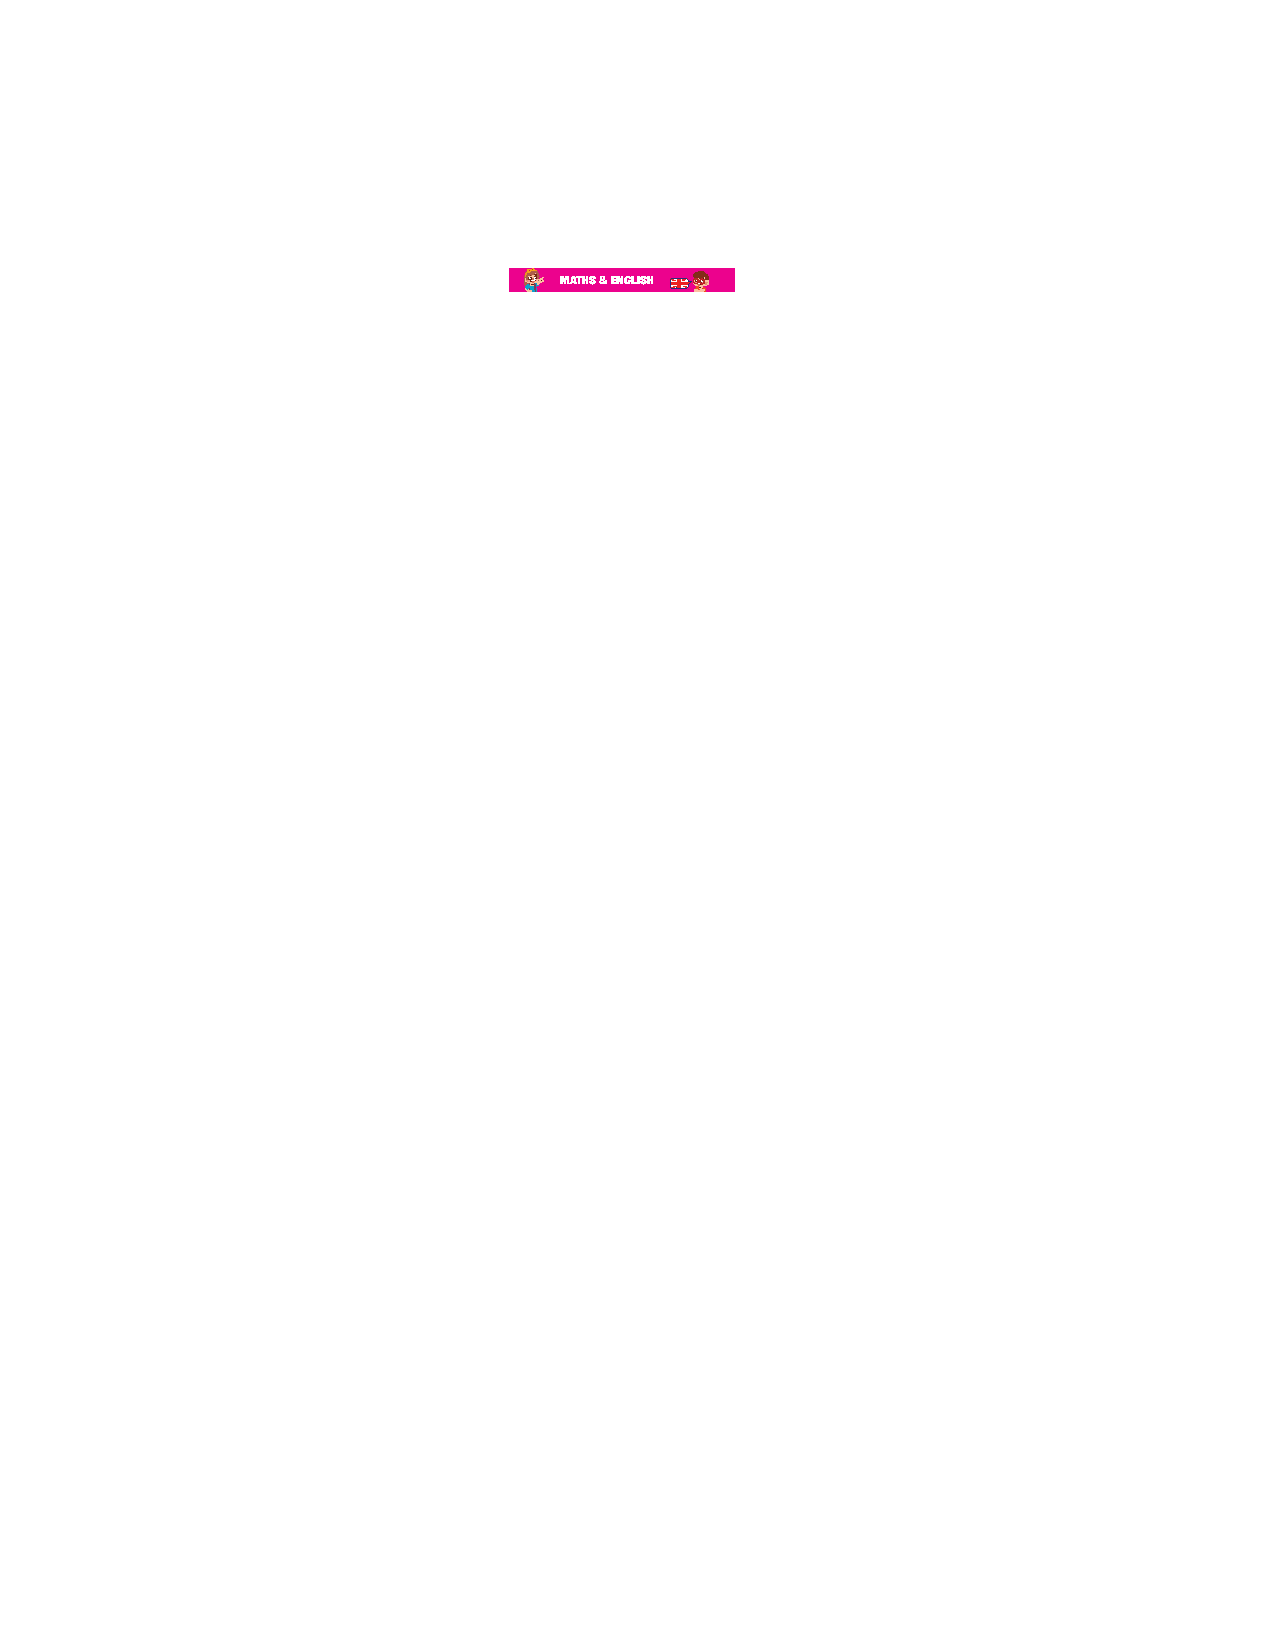
\includegraphics[width=17.2cm]{../mathc.pdf}}}
%\AddToShipoutPicture*{\put(-2,733){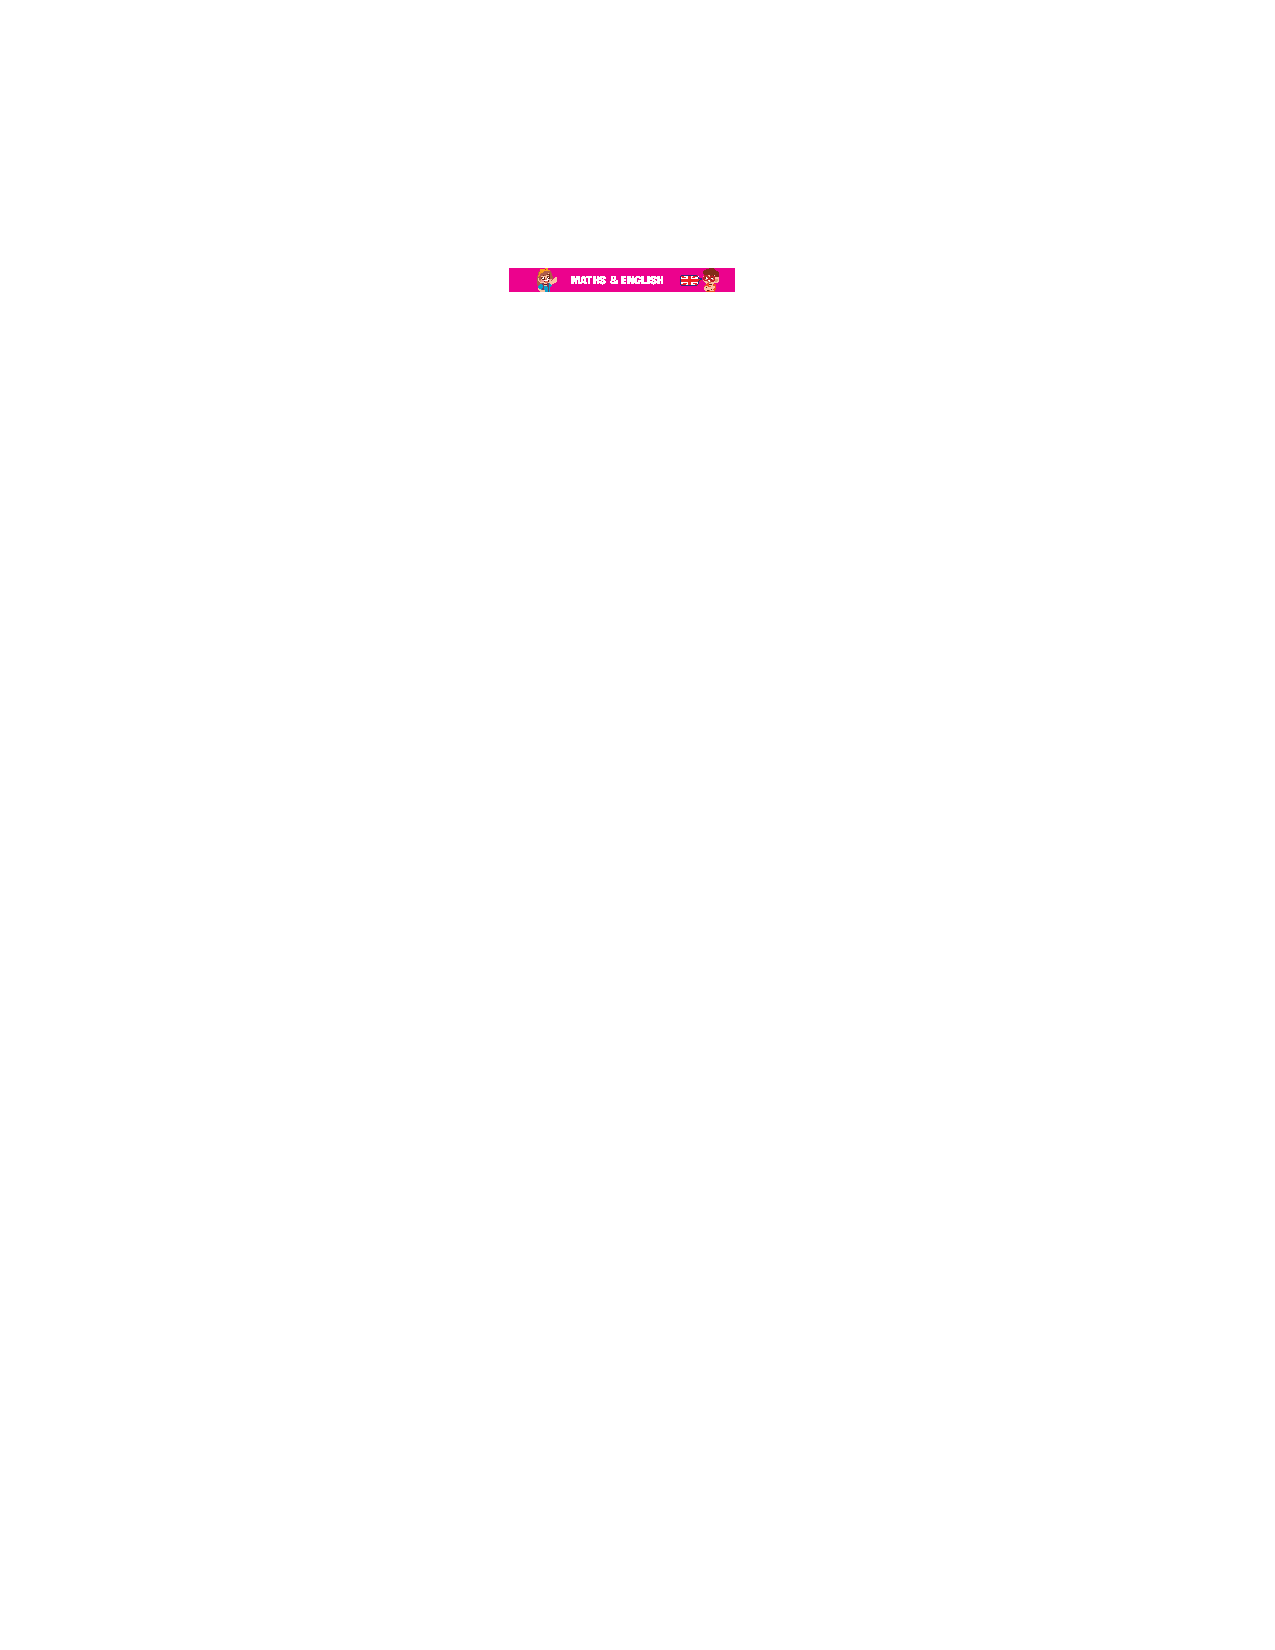
\includegraphics[width=17.2cm]{../mathl.pdf}}} 
\AddToShipoutPicture*{\put(189,675){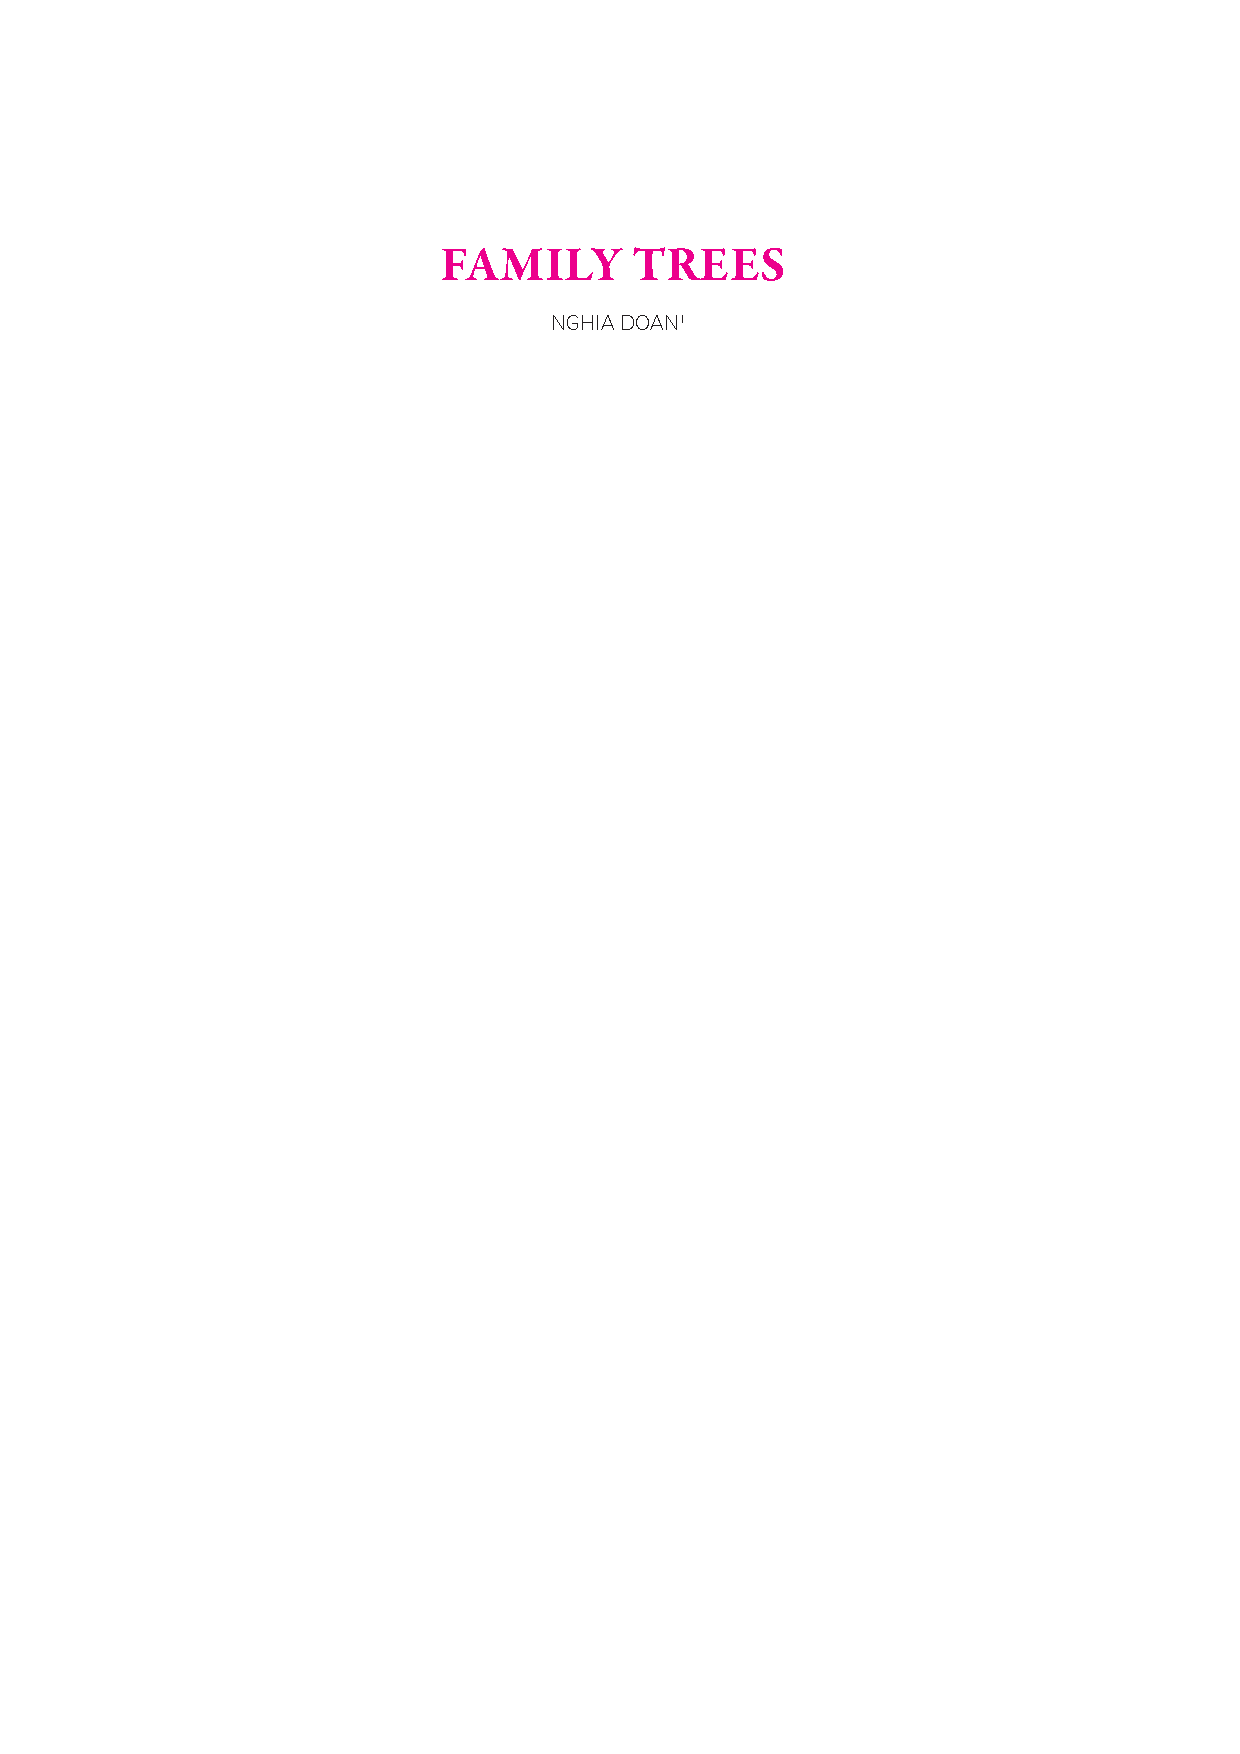
\includegraphics[scale=1]{../tieude4.pdf}}} 
\centering
\endgroup
\graphicspath{{../toancuabi/pic/}}
\vspace*{30pt}

\begin{multicols}{2}
	Below you see an example of \textit{family tree}.
	The circles denote female members and the triangles males.
	\begin{figure}[H]
		\vspace*{-5pt}
		\centering
		\captionsetup{labelformat= empty, justification=centering}
		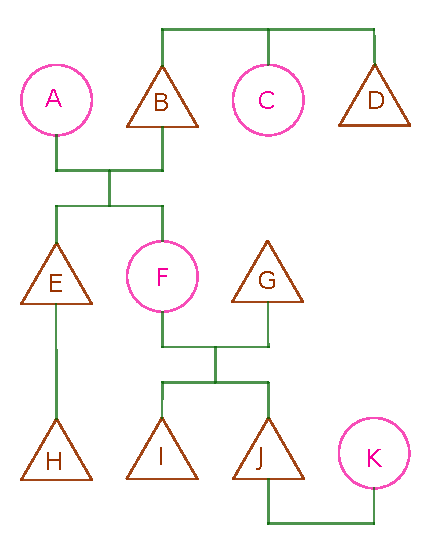
\includegraphics[width= 0.75\linewidth]{hc-2022-2-3-15-1.pdf}
		\vspace*{-10pt}
	\end{figure}
	$A$ and $B$ are married, as are $F$ and $G,$ and $J$ and $K.$
	\vskip 0.1cm
	$B, C,$ and $D$ are siblings, as are $E$ and $F.$
	$E$ and $F$ are children of $A$ and $B.$
	\vskip 0.1cm
	Similarly, the parents of $I$ and $J$ are $F$ and $G.$
	$E$ is the father of $H.$
	\vskip 0.1cm
	In addition, $A$ is the grandmother of $H, I,$ and $J,$
	$F$ is the aunt of $H,$ and $C$ is the sister--in--law of $A.$
	\begin{figure}[H]
		\vspace*{-5pt}
		\centering
		\captionsetup{labelformat= empty, justification=centering}
		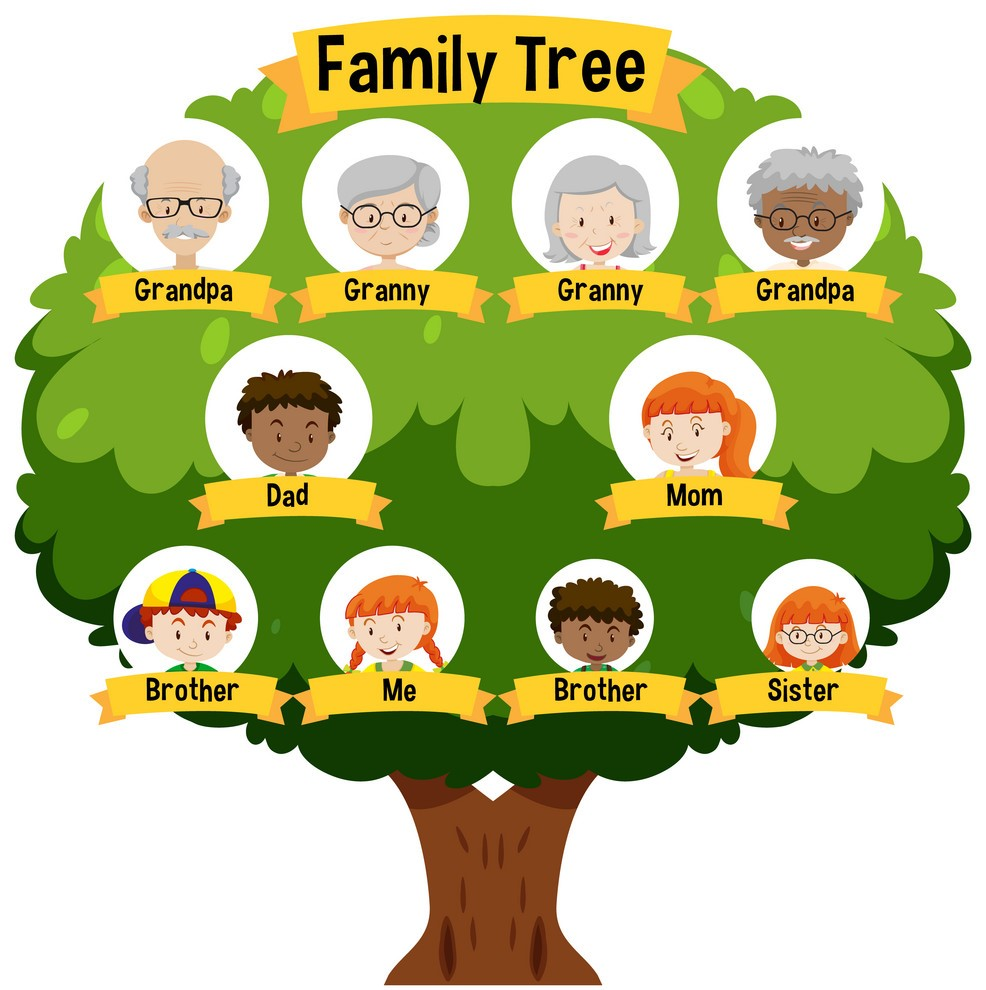
\includegraphics[width= 0.92\linewidth]{tree1}
		%		\vspace*{-5pt}
	\end{figure}
	
	\vspace*{0.1pt}
	
	\vspace*{-7pt}
	\PIbox{
		{\color{toancuabi}\textbf{Example} (Who are who)\textbf{.}}
		Inspector Jade asked six children to briefly introduce their brothers, sisters,
		and first cousins (cousins who share a grandparent.)
		She had to match the name of the child to each numbered position in the family tree
		with the responses as below. Note that the relations given are in local languague.
		\textit{Do not try to guess the genders of the children from the names. It might lead you to the wrong way.}
		\vskip 0.1cm
		Response from Binh:
		\vskip 0.1cm
		$\circ$ I have three \textit{arawa}: Kim, Minh, Thao
		\vskip 0.1cm
		$\circ$ I have two \textit{surubu}: Oanh and Yen
		\vskip 0.1cm
		Response from Dinh:
		\vskip 0.1cm
		$\circ$ I have two \textit{surubu}: Oanh and Yen
		\vskip 0.1cm
		$\circ$ I have one \textit{ere}: Binh
		\vskip 0.1cm
		Response from Kim:
		\vskip 0.1cm
		$\circ$ I have one \textit{arawa}: Dinh
		\vskip 0.1cm
		$\circ$ I have one \textit{surubu}: Binh
		\vskip 0.1cm
		Response from Minh:
		\vskip 0.1cm
		$\circ$ I have one \textit{ere}: Yen
		\vskip 0.1cm
		$\circ$ I have two \textit{arawa}: Dinh and Thao
		\vskip 0.1cm
		Response from Thao:
		\vskip 0.1cm
		$\circ$ I have two \textit{surubu}: Yen and Binh
		\vskip 0.1cm
		$\circ$ I have two \textit{arawa}: Minh and Dinh}
	\begin{figure}[H]
		\vspace*{-5pt}
		\centering
		\captionsetup{labelformat= empty, justification=centering}
		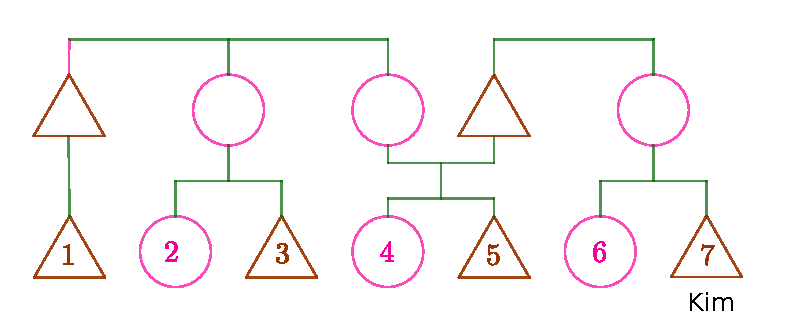
\includegraphics[width= 1\linewidth]{hc-2022-2-3-15-2.pdf}
		\vspace*{-20pt}
	\end{figure}
	\textit{Solution.} From what Binh said, Binh has the same type of relations to three children.
	Thus, those cannot be Binh's sisters or brothers,
	and \textit{arawa} does not mean sister or brother.
	Only the child number $4$ or $5$ has three cousins in the same gender.
	\vskip 0.1cm
	Look at the cousins of the children $4$ or $5,$
	\textit{arawa} or \textit{suburu} rather related to the gender of the cousin
	than the gender of the cousin's father or the mother.
	Note that Binh is a \textit{suburu} to Kim and Kim is an \textit{arawa} to Binh.
	Thus, Binh and Kim are of opposite genders, so Binh is a girl.
	Hence, Binh is the girl number $4.$
	\vskip 0.1cm
	Therefore, Kim, Minh, and Thao are the children $1, 3,$ and $7,$
	and \textit{arawa} means \textit{male cousin(s).}
	Furthermore, Binh is a \textit{suburu} to Kim and Thao,
	in other words, she is a \textit{female cousin} to them.
	\vskip 0.1cm
	This means that Binh is not a \textit{suburu} to the boy $5.$
	Obviously, she is not an \textit{arawa} to anyone.
	Since she is an \textit{ere} to Dinh, Dinh must be her brother.
	Thus Dinh is the boy number $5.$
	\vskip 0.1cm
	Now, Thao must be the boy number $1$ because he has two female and two male cousins.
	That leaves Minh must be the boy number $3.$
	\vskip 0.1cm
	Yen is a \textit{ere} to Minh, so Yen is the girl number $2.$
	Finally, Oanh is the girl number $6.$
	\vskip 0.1cm
	The answer is $1-$Thao, $2-$Yen, $3-$Minh, $4-$Binh, $5-$Dinh, $6-$Oanh, $7-$Kim.
	\vskip 0.25cm
	\PIbox{
		\centerline{\textbf{\color{toancuabi}Vocabulary}}
		\vskip 0.1cm
		{\color{toancuabi}male}: nam
		\vskip 0.1cm
		{\color{toancuabi}female}: nữ
		\vskip 0.1cm
		{\color{toancuabi}family tree}: cây phả hệ 
		\vskip 0.1cm
		{\color{toancuabi}sibling}: anh/chị/em ruột 
		\vskip 0.1cm
		{\color{toancuabi}aunt}: cô, dì 
		\vskip 0.1cm
		{\color{toancuabi}sister--in--law}: chị/em dâu 
		\vskip 0.1cm
		{\color{toancuabi}cousin}: anh/chị/em họ 
		\vskip 0.1cm
		{\color{toancuabi}gender}: giới tính 
	}
\end{multicols}
\begin{figure}[H]
	\vspace*{-5pt}
	\centering
	\captionsetup{labelformat= empty, justification=centering}
	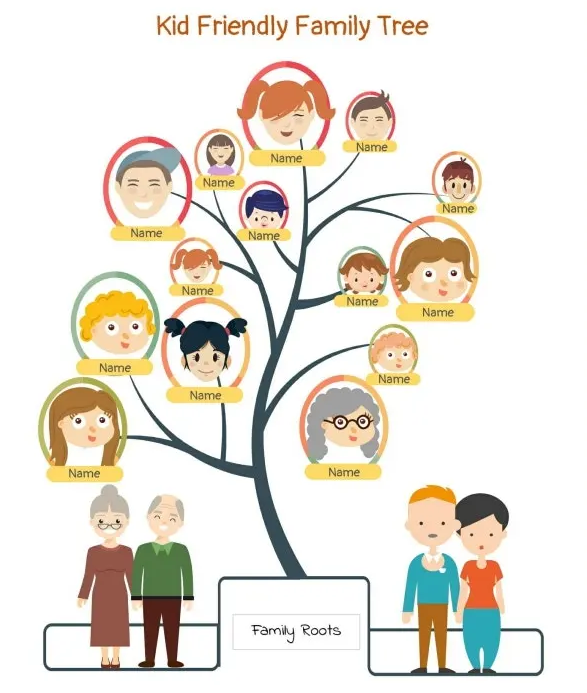
\includegraphics[width= 0.65\linewidth]{tree2}
	\vspace*{-5pt}
\end{figure}